\documentclass[12pt,a4paper]{article}

% Margins.
\setlength{\oddsidemargin}{0in}
\setlength{\evensidemargin}{0in}
\setlength{\headheight}{12pt}
\setlength{\headsep}{42pt}
\setlength{\topmargin}{-54pt}
\setlength{\textwidth}{6.5in}
\setlength{\textheight}{10in}

\usepackage{amsmath}
\usepackage{float}
\usepackage{graphicx}
\usepackage[hyphens]{url}
\usepackage{hyperref}	% Clickable links to figures, references and urls.
\usepackage{datetime}
\usepackage{longtable}
\usepackage{subfigure}

% Links direct to top of figures.
\usepackage[all]{hypcap}

% Drawing.
\usepackage{pgf}
\usepackage{tikz}

% Listings for formatting code.
\usepackage{listings}
\usepackage{textcomp}
% General options.+++
\lstset{breaklines=true, basicstyle=\small\ttfamily, tabsize=4, numbers=left, stepnumber=1, frame=single, showstringspaces=false, upquote=true}
% C++ specific high-lighting. Comments are 50/50 shades of green/black and strings coloured with 60/40 red/black mixture.
\lstset{language=[ISO]C++, commentstyle=\color{green!50!black}, keywordstyle=\color{blue}, stringstyle=\color{red!60!black}}

%opening
\title{\vspace{-3cm}Physics for Engineers\\Class 25\\Conductors in Electrostatic Equilibrium}
\author{Attique Dawood}
\date{October 21, 2013\\[0.2cm] Last Modified: \today, \currenttime}
\begin{document}
\maketitle
\section{Announcements}
\begin{itemize}
\item Assignment 05 due today.
\item Quiz \#05 today.
\end{itemize}
\section{Conductors in Electrostatic Equilibrium}
What happens if you place two charges near each other and then leave them? If the charges are free to move they both will experience an electrostatic force. When will the charges stop moving, i.e., when will they be in equilibrium? The charges will move far away from each other until they no longer experience any force.

Now assume the charges are free to move only in a particular region. How can they be in equilibrium? Only if they keep maximum distance from each other. What about three charges? They will position themselves on the boundary of the region because this is the only place where they can keep maximum distance from each other.

This is exactly how charges behave when they reside on a conductor. Charges can freely move in a conductor but they cannot leave the boundary of the conductor. The only place they can go is the surface of the conductor. \textbf{Free charges on a conductor will always move to the surface of the conductor so as to establish a state of equilibrium}. Another fact about conductors is that \textbf{electric field inside a conductor is zero at all times}.
\section{Exercises}
\noindent\textbf{Question 1:} A spherical conductor of radius $R$ has total charge $q$. Use Gauss's Law to find electric field everywhere.\\[0.2cm]
\noindent\textbf{Question 2:} A conducting shell exists at $r=a$ to $r=b$. Space inside the shell is free space. If a charge $q$ is placed at the centre of the shell find electric field everywhere.\\[0.2cm]
\noindent\textbf{Question 3:} A conducting shell exists at $r=a$ to $r=b$ and has a net charge $2q$. Space inside the shell is free space. If a charge $-q$ is placed at the centre of the shell find electric field everywhere.\\[0.2cm]
\noindent\textbf{Question 4:} A uniform charge density $\rho_v$ exists in the region from $r=a$ to $r=b$. Find electric field everywhere. Note: There is no conductor here, only charge in free space.\\[0.2cm]
%\begin{itemize}
%\item[a.] Electric field of a point charge.
%\item[b.] Electric field of an infinite line charge placed along $z$--axis.
%\end{itemize}
%%\begin{figure}[H]
%\centering
%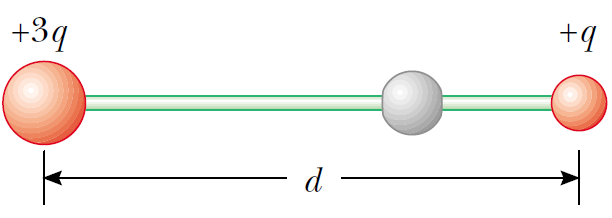
\includegraphics[scale=0.45]{FigureP23-10.png}
%\caption{Equilibrium of charge.}
%\label{Equilibrium}
%\end{figure}
%\nocite{*}
%\bibliographystyle{plain}
%\bibliography{PhysicsRef}
\end{document}
